


\chapter{Grundlagen}\label{basics}
\section{Fazialisparese und House-Brackmann Skala}\label{facialpalsy}
\paragraph{Fazialisparese} (eng. Facial nerve Paralysis) ist eine Funktiosstörung der Hirnnerven und der mimischen Gesichtsmuskulatur. Durch diese Nervenbahnstörung können eine partielle oder auch vollständige Beeinträchtigung der Muskeln im Gesicht ausgeprägt sein. Dabei werden vor allem der Lidschluss, Strinbewegungen (runzeln und Augenbraun heben), Mundwinkel und Lippenschluss als offensichtliche Merkmale negativ beeinflusst. Auch können Geschmack, Hörsinn, Speichel und Tränenfluss in Mitleidenschaft gezogen sein \cite{facialpalsy_1}\cite{facialpalsy_2}.

Liste von Ursachen für die Ausprägung einer Fazialisparese:
\begin{itemize}
  \setlength\itemsep{-0.5em}
\item Infektionen (z.B. Borrelien)
\item Entzündungen
\item Traumatische oder geburtstraumatische
Schädigung
\item Tumore
\item Angeborener Defekt
\item Idiopathisch (Bell-Parese)
\item Verletzung des Nerves
\end{itemize}

Es gibt verschiedenste Skalen, die eine Einordung für den Schwereverlauf einer vorhandenen Fazialisparese, realisieren. Die bekanntesten Skalen sind dabei Sunnybrook und die House-Brackmann Skala. Im Rahmen der Bachelorarbeit wird allein die House-Brackmann Skala zur Anwendung kommen. Diese ist im Vergliech zur den anderen Skala einfacher im Umgang und der Späteren Ausgabe. Auch ist diese aus medizinischer Sicht ein Standart zur Bewertung der Schwere.




\paragraph{House-Brackmann Skala} ist ein Score der für die Ermittlung des Schweregrades der Fazialisparese Anwendung findet, der von John W. House und Derald E. Brackmann 1983 eingeführt wurde. Das Sytsem beinhaltet eine 6-Punkte Skala von römisch I Normalzustand bis IV vollständig ausgeprägte Parese (Tabelle \ref{cap:housebrackmann}). Die Einstufung erfolgt, indem der Patient aufgefordert wird, bestimmte Bewegungen auszuführen. Diese werden durch einen Facharzt*in klinisch beobachtet und eine subjektive Beurteilung der Schwere der vorliegenden Parese zuordnet \cite{housebrackmann}.

Vorteil dieser Skala besteht durch die einfache Handhabung und darin, dass sie anhand einzelner Figuren die Beschreibung der Gesichtsfunktion erfolgen kann.
Nachteilhaft sind dabei die subjektieve Bewertung des/dem behandeltem Arzt*in und die reginoalen Funktionsunterschiede zwischen dem Grad III und V unempfindlicher für Veränderungen sind.

\begin{table}[!tb]\vspace{1ex}\centering
  \resizebox{0.85\textwidth}{!}{
  \small
  \begin{tabular*}{15.5cm}{c||c|cccc|}
%\hline
\multirow{2}{*}{\textbf{Grad}} &
  \multirow{2}{*}{\textbf{Beschreibung}} &
  \multicolumn{1}{c|}{\textbf{Statisch}} &
  \multicolumn{3}{c|}{\textbf{Dynamisch}} \\ \cline{3-6}
 &
   &
  \multicolumn{1}{c|}{\textbf{Symmetrie}} &
  \multicolumn{1}{c|}{\textbf{Stirn}} &
  \multicolumn{1}{c|}{\textbf{Lidschluss}} &
  \textbf{Mund} \\ \hline\hline
I &
  Normal &
  \multicolumn{4}{c|}{Normal} \\ \hline
II &
  \begin{tabular}[c]{@{}c@{}}Leichte\\ Funktionsstörung\end{tabular} &
  \multicolumn{1}{c|}{Normal} &
  \multicolumn{1}{c|}{\begin{tabular}[c]{@{}c@{}}moderate\\ bis\\ gute\\ Funktion\end{tabular}} &
  \multicolumn{1}{c|}{\begin{tabular}[c]{@{}c@{}}geschlossen,\\ minimale\\ Anstrengung\end{tabular}} &
  \begin{tabular}[c]{@{}c@{}}leichte\\ Asymmetrie\end{tabular} \\ \hline
III &
  \begin{tabular}[c]{@{}c@{}}Moderate\\ Funktionsstörung\end{tabular} &
  \multicolumn{1}{c|}{Normal} &
  \multicolumn{1}{c|}{\begin{tabular}[c]{@{}c@{}}leicht\\ bis\\ moderate\\ Funktion\end{tabular}} &
  \multicolumn{1}{c|}{\begin{tabular}[c]{@{}c@{}}geschlossen,\\ maximale\\ Anstrengung\end{tabular}} &
  \begin{tabular}[c]{@{}c@{}}leicht Betroffen,\\ maximale\\ Anstrengung\end{tabular} \\ \hline
IV &
  \begin{tabular}[c]{@{}c@{}}Mittelschwere\\ Funktionsstörung\end{tabular} &
  \multicolumn{1}{c|}{Normal} &
  \multicolumn{1}{c|}{keine} &
  \multicolumn{1}{c|}{unvollständig} &
  \begin{tabular}[c]{@{}c@{}}Asymmetrisch,\\ maximale\\ Anstrengung\end{tabular} \\ \hline
V &
  \begin{tabular}[c]{@{}c@{}}Schwere\\ Funktionsstörung\end{tabular} &
  \multicolumn{1}{c|}{Asymmetrisch} &
  \multicolumn{1}{c|}{keine} &
  \multicolumn{1}{c|}{unvollständig} &
  \begin{tabular}[c]{@{}c@{}}leichte\\ Bewegung\end{tabular} \\ \hline
VI &
  komplette Parese &
  \multicolumn{4}{c|}{keine} \\ \hline
  \end{tabular*}
  }
  \caption[Schweregradeinteilung der Fazialisparese nach House-Brackmann]{Schweregradeinteilung der Fazialisparese nach House-Brackmann von Grad I, keine sichtbaren Auswirkungen der Parese , bis Grad VI vollständing ausgeprägte Parese \cite{housebrackmann}.}\label{cap:housebrackmann}
\vspace{2ex}\end{table}\label{table:housebrackmann}


\section{Maschinelles Lernen und Neuronale Netze}\label{neuralnet}
\paragraph{Maschinelles Lernen} ist ein Teilgebiet der Künstlichen Intelligenz umfassd im Allgemeinen, durch Methoden und Lernporzesse Zusammenhänge in Datensätzen zu erkennen. Darauf basierend sollen Vohersagen getroffen werden. Ein Optimierungsproblem soll so gelöst werden, das aus einer Korrelation zwischen einem Ausgabewert und der Eingabe besteht. Durch selbstlernende Algroithmen sollen diese Modelle die Vorhersagegenauigkeit selber anpassen und den Ausgabewert in der Genauigkeit verbessern, ohne dabei den Algorithmus explizit zu programmieren zu müssen \cite{machinelearning_1} \cite{machinelearning_2}.

Diese  Lernverfahren können in drei Kategorien aufgeteilt werden:
\begin{itemize}
  \setlength\itemsep{-0.5em}
\item Überwachtes Lernen
\item Unbewachtes Lernen
\item Bestärkendes Lernen
\end{itemize}

Bei dem überwachten Lernverfahren wird das Modell trainiert, um ein Ausgabewert eines nicht bekannten Datensatzes (Validations-Datensatz) verhergesagt werden kann. Ziel ist die Genauuigkeit dieser Vorhersage zu maximieren. Das Gegenteil davon das unbewachte Verfahren. Dabei die Ausgabe nicht bekannt oder es kann keine präzise Aussage darüber getroffen werden. Anhand der Eingabe sollen so Muster und Zusammenhäne herausgefunden werden. Bestärkendes Lenen, beschreibt eine Methode, womit das Modelll bestraft, oder belohnt wird um ein Ergebnis zu optimieren \cite{machinelearning_1}.

Im Verlauf dieser Arbeit wird nur das \textbf{überwachte Lernen} der Modelle betrachtet.


\paragraph{Neuronale Netze} werden vor allem für die Klassifikation von Daten und Regression eingesetzt. Hierbei werden Parameter des Netzes optimeirt, die zwischen den einzelnen Schichten (eng. Layer) liegen. Nicht-Lineare Aktivierungsfunktionen transformieren Eingabewerte in andersliegende Wertebereiche. Ergebnisse dieser Funktion dienen in weiterführende Schichten als Eingabe (Abb. \ref{cap:neuralnet}). Diese Layer können auch eine diskrete Faltung oder eine Normalisierung dieser Schichten darstellen. In Kombination mit der Verschachtelung der verschiedensten Layerarten können so belibig komplizierte Modelle gebildet werden \cite{machinelearning_3}.


\def\layersep{2.5cm}
\begin{figure}[!tb]\centering
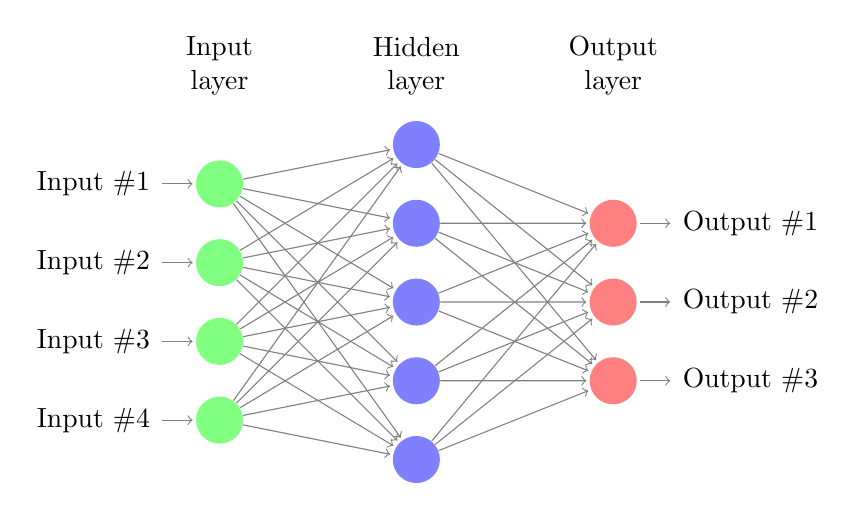
\begin{tikzpicture}[shorten >=1pt,->,draw=black!50, node distance=\layersep]
    \tikzstyle{every pin edge}=[<-,shorten <=1pt]
    \tikzstyle{neuron}=[circle,fill=black!25,minimum size=17pt,inner sep=0pt]
    \tikzstyle{input neuron}=[neuron, fill=green!50];
    \tikzstyle{output neuron}=[neuron, fill=red!50];
    \tikzstyle{hidden neuron}=[neuron, fill=blue!50];
    \tikzstyle{annot} = [text width=4em, text centered]

    % Draw the input layer nodes
    \foreach \name in {1,...,4}
        \node[input neuron, pin=left:Input \#\name] (I-\name) at (0,-\name) {};

    % Draw the hidden layer nodes
    \foreach \name in {1,...,5}
        \path[yshift=0.5cm]
            node[hidden neuron] (H-\name) at (\layersep,-\name cm) {};

    % Draw the input layer nodes
    \foreach \name in {1,...,3}
      \node[output neuron, pin={[pin edge={->}]right:Output \#\name}] (O-\name) at (2*\layersep,-0.5cm-\name cm) {};

    % Connect every node in the input layer with the hidden layer.
    \foreach \source in {1,...,4}
        \foreach \dest in {1,...,5}
            \path (I-\source) edge (H-\dest);

    % Connect every node in the hidden layer with the output layer
    \foreach \source in {1,...,5}
        \foreach \dest in {1,...,3}
            \path (H-\source) edge (O-\dest);

    % Annotate the layers
    \node[annot,above of=H-1, node distance=1cm] (hl) {Hidden layer};
    \node[annot,left of=hl] {Input layer};
    \node[annot,right of=hl] {Output layer};
\end{tikzpicture}
\caption[Beispielaufbau eines Neuronale Netzes]{Beispielaufbau eines Neuronale Netzes. Die Input Layer repräsentieren die Eingabe in das Netz. Hidden Layer sind versteckte Schichten im Modell. Die Ausgabe auf der linken Seite sind bei einer Klassifikation Wahrscheinlichkeiten, bezogen auf die  zu erwartenden Label. Die Kanten zwischen den Schichten haben Gewichte ahand deren die Eingabe modifiziert wird.}\label{cap:neuralnet}
\end{figure}\label{fig:neuralnet}

Das Training dieser Netze basiert auf Forwärts- und Rückwärtsrechnen dier Geichte und Parameter an den Kanten. Dabei läuft zuerst die Eingabe des neuronalen Netzes alle Schichten, die eine Reihe von Transformationen ausführt. Das Ergebnis nach den Durchlauf wird mit dem realen Ergebnis verglichen, das innerhalb der Trainingsphase bekannt ist. Die Abweichung von diesem Vergleich, auck bekannt als Fehler, wird in der umgekehrten Richtung durch das Netzwerk geschickt. Die Gewichte an den Kanten zwischen den Layern werden anhand des Fehlers angepasst. So soll erreicht werden, dass das Netz sich im Verhalten der Ein- und Ausgabe konvergiert.

\section{Automatentheorie}\label{automatatheory}
\textbf{TODO}

\section{Statistik}\label{statistics}
\textbf{Erklären wie man die ausrechnet über Confusion Matrix}



here Recall refers to as true positive rate (tpr), and
Confidence denotes the true positive accuracy (tpa). Consid-
ering all four metrics rather than only an accuracy can help
to reduce the evaluation bias to an extent.


\textbf{Treffergenauigkeit}
\begin{equation}
Treffergenauigkeit (ACC) = \frac{TP+TN}{TP + TN + FP + FN}
\end{equation}

\textbf{Sensitivity, hit rate, recall, or true positive rate}
\begin{equation}
Sensitivität (TPR) = \frac{TP}{TP + FN}
\end{equation}

\textbf{Precision or positive predictive value}
\begin{equation}
Genauigkeit (PPV) = \frac{TP}{TP + FP}
\end{equation}

\textbf{F1}
\begin{equation}
F1 = \frac{2 * PPV * TPR}{PPV + TPR} = \frac{2 * TP}{2 * TP + FP + FN}
\end{equation}


























\chapter{Stand der Technik}\label{std}

Im folgenden Kapitel soll der momentane  Stand der Technik für die zugrunge liegende Aufgabenstellung erläutert werden. Der Abschnitt \ref{segmentation} veranschaulicht dabei die Graduierung der Fazialisparese duch die Anwendung von Segmentierung zur Extraktion der wichtigsten Gesichtseigenschaften.
\textbf{TODO}

\section{Segmentierung basierte Methode}\label{segmentation}
Eine Methode zur Erkennung einer Fazialisparese ist die Anwendung von Segmentierung, um die Gesichtsmerkmale aus den Bildern extrahierten. Diese semantischen Merkmale enthalten räumliche Eigenschaften des Patienten*in, die für die Klassifikation des Schweregrades, aus optischer sicht, unerlässlich sind.

\begin{figure}[tb]\centering
  %width=0.98\textwidth
  \includegraphics[width=15cm]{./images/wang1-2942143-large.eps}
\caption[tmp2]{TODO NEU ZEICHNEN\cite{detection_fp2}}\label{cap:tmp2}
\end{figure}\label{fig:tmp2}

Der Experimentaufbau von T. Wang, S. Zhang, L. Liu, G. Wu und J. Dong enthaltet ein kaskadierenden Encoder Netzstruktur zur Ausführung der Bewertung der Fazialisparese. Auf Basis von Neuronalen Netzen, besteht dieser Aufbau aus zwei Komponenten. Semantischen Segmenterung von Gesichtsattributen und ein Klassifikationsnetz über eine vorher extrahierte Funktionskarte (Encoder). Dieser Encoder komprimiert die Bilddaten Pixel für Pixel durch ein Faltungsnetzwerk (eng. Convolution). Verwendet wird dazu ein vortrainiertes ResNet-101 ohne Verkleinerung des Eingabemateriales. Als Training für für den Encoder diente ein Mix aus beiden, normale und an einer Fazialisparese leidenden Personen, um ihn seperat vom Rest vorab zu trainieren. Daturch konnte genug räumliche Informationen über die Gesicher gewonnen werden, die für die Segmenterung und die Graduierung benötigt werden. Die daraus enthaltenen Daten aus dem Encoder dienen als Feature für die Segmentierung und die direkte Klassifikation des Grades nach House-Brackmann. Segmentierung ist eine Pixel für Pixel Klassifikation über das gesammte Bild. Die Gesichtspartien können so für die betrachteten Teilregionen der House-Brackmann Skala eingefärbt werden. Als Ausgabe dient die Klassifizerung und das segmentierte Bild, der für die weitere klinische Einschätzung durch einen Facharzt*in zurückgeliefert werden. Durch die Anwendung des kaskadierenden Trainings ist so ein F1 Wert von 95.85\% erzielt \cite{detection_fp2}.




\section{Vergleichsbasiert}\label{compare}
Eine anderweitige Möglichkeit ist es mit einem Video Frames mit einer Referenz zu vergleichen. Dazu werden fünf unterschiedlichste Gesichstbewegungen durchgeführt. Diese sind Augenbraun heben, Augen sanft und forciert schließen, Nase rümpfen und Lächeln. Die Viedeosequenz beginnt mit der Referenzansicht, wobei sich der/die Patient*in in Ruheposition befindet. Nach jeder Bewegung kehren sie auch wiederum in die Ausgangsposition zurück. Anhand von Framesubstraktion können die einzelnen Positionen aus dem Video entnommen werden.

Nachdem die einzelnen Posen entnommen worden sind werden die einzelnen Gesichtsregionen lokalisiert. Um die Gesichskonturen zu detektieren wird ein Sobel-Filter angewendet. Dieser nutzt eine Faltungsoperation, die aus dem Bild einen Gradienten erzeugt. Die Bereiche mit der größten Intensität, also den Stellen wo sich die Helligkeit am stärksten ändert, werden hervorgehoben. Die anderen Stellen werden mit Grauwerten drargestellt. Alle eintscheidenden Features des Gesichtes (Augenbraun, Nase, Mund und Augen) sind dunkler als die normale Hautfarbe. Durch Eine Verschiebung der Pixelwerte lassen sich diese hervorheben und deren absolute Position im Bild feststellen.

Anhand dessen werden 4 Eingabewerte berechnet, die für eine Klassifikation mit einem Neuronalen Netz benötigt werden. Dazu zählen die relative Pixeländerung in den einzelnen Regionen, die sich von der Ruheposition bis zu dem Höhepunkt der dargestellten Bewegung ausgerechnet wird. Auch der Beleuchtungskompensationsfaktor, der die Unterschiede zwischen der dysfunktionalen und der normalen Seite betrachtet, um die Intensität und Ausprägung der Funktionsstötung ermittelt. Die anderen beiden sind Faktoren die sich aus dem optischen Fluss der Regionen darstellen lässt. Dazu werden Vektoren genutzt die von der Spiegelachse - Nasenrücken - beide Gesichtshäften in einem Raster die Richtungsänderungen und Falten im Gesicht zeigen sollen. Aus dieser Grafik werden einmal die Symmetrie in vertikaler Richtung und die Stärke dieser Vektoren berechnet. Diese genannten Fatoren dienen als Eingabe in ein Klassifikationsnetzwerk, dass nach der House-Brackmann Skala den Grad der Parese feststellt \cite{detection_fp1}.

\textbf{TODO, kleines Bild zeichnen ?? Eingabe (4 Faktoren zeichnen + Formel?) -> Netz -> Ausgabe}
